\documentclass{article}
\usepackage[utf8]{inputenc}
\usepackage[spanish]{babel}
\usepackage{listings}
\usepackage{graphicx}
\graphicspath{ {images/} }
\usepackage{cite}

\begin{document}

\begin{titlepage}
    \begin{center}
        \vspace*{1cm}
            
        \Huge
        \textbf{Proyecto Final}
            
        \vspace{0.5cm}
        \LARGE
        Juego
            
        \vspace{1.5cm}
            
        \textbf{Santiago Pereira Ramirez}
            
        \vfill
            
        \vspace{0.8cm}
            
        \Large
        Despartamento de Ingeniería Electrónica y Telecomunicaciones\\
        Universidad de Antioquia\\
        Medellín\\
        Septiembre de 2021
            
    \end{center}
\end{titlepage}

\tableofcontents
\newpage
\section{Idea}\label{intro}
Hace algunos años aliens llegaron al planeta tierra a destruir la especie humana, luego de grandes guerras contra los aliens.Estos casi logran destruir a la humanidad pero nuestro gran justiciero alienkiller ha encontrado una debilidad, ahora su proposito es llegar a una de las tantas bases de la resistencia para compartir la informacion y combatir juntos a los extraterrestres.

\section{Personajes,enemigos e items} \label{intro}

--Nuestro personaje principal tendra su arma especial la cual le permitira destruir a sus enemigos.\\

--Los diversos enemigos iran para combatir a nuestro pretagonista los cuales tendran movimientos lo cual dificultara la pelea.\\

--los items  se podran visualizar cuando se elimine a algun enemigo, se podra recuperar vida,perder vida, o aumentar la velocidad del personaje.


\section{Entorno} \label{intro}

--En uno de los niveles alienkiller debera de robar una nave enemiga y destruir un batallon que llega a apoyar a extraterrestres asentados en el planeta tierra.\\

\begin{figure}[h]
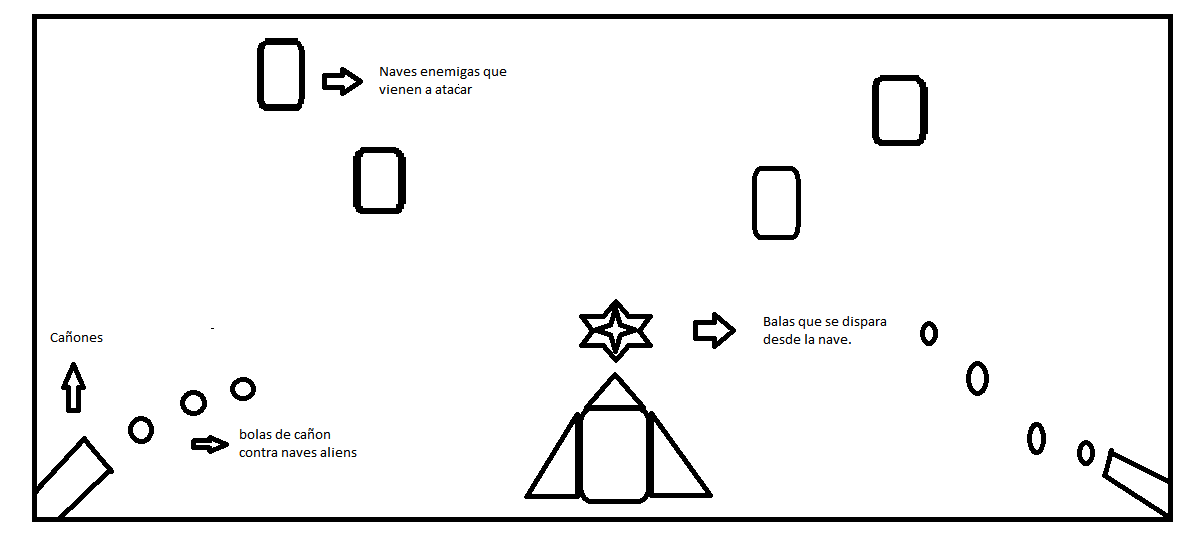
\includegraphics[width=17cm]{Nivel_1.PNG}
\centering
\end{figure}


\\--Otro de los niveles el personaje debera de matar a los enemigos a travez de las balas lanzada desde sus armas y esquivando enemigos con movimientos particulares.

\begin{figure}[h]
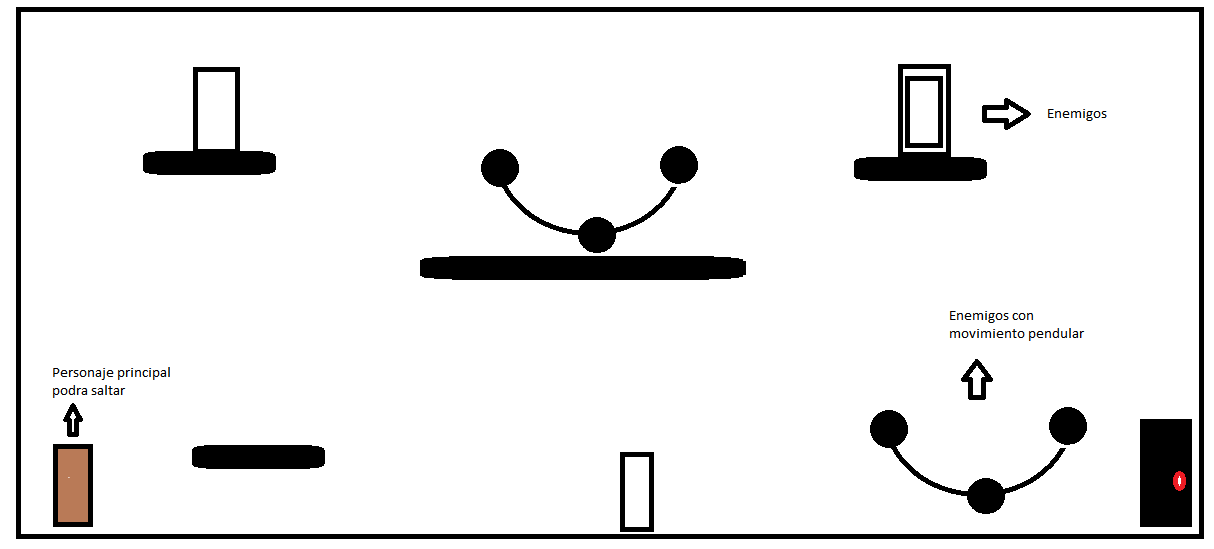
\includegraphics[width=14cm]{Nivel_2.PNG}
\centering
\end{figure}

\section{Clases} \label{intro}

--bosquejos de lo que seran las clases


1)\\
class alienkiller\\
{\\
private:\\
    float vida;\\
    float daño;\\
    float posicion_x;\\
    float posicion_y;\\
    float velocidad;\\
    float coeficientes;\\
    float angulo;\\
    
        
public:\\
    alienkiller(float pos_x,float pos_y);\\
    void calcular_posicion();\\
    void calcular_variables();\\
    void dar_forma();\\
    
};\\

2)\\
class Bala\\
{\\
private:\\
    float velocidad;\\
    float angulo;\\
    float velocidad_x;\\
    float velocidad_y;\\
    float posicion_x;\\
    float posicion_y;\\
    float daño; \\
    float delta_tiempo;\\
    float gravedad;\\
    
public:\\
    Bala();\\
    void calcular_variables();\\
    void calcular_posicion();\\
    void dar_forma();\\
    
};\\

3)\\
class Enemigos\\
{\\
private:\\
    float vida;\\
    float  daño;\\
    float  posicion_x;\\
    float  posicion_y;\\
    float  velocidad;\\
    float Angulo;\\
    
    
public:\\
    Enemigos(float pos_x,float pos_y);\\
    void  calcular_posicion();\\
    void  calcular_variables();\\
    void  dar_forma();\\
};\\

\end{document}
